\chapter{Reglerentwurf} \label{ch_Reglerentwurf}
In diesem Kapitel werden die Eigenschaften des zu regelnden Modells vorgestellt und darauf aufbauend dessen Ein- und Ausgangsgrößen festgelegt.
Anschließend wird ein geeigneter Regler vorgestellt und der resultierende Regelkreis abgeleitet.
Zuletzt wird die Übertragbarkeit der Regelung auf das Realsystem des Solarturmkraftwerkes in Jülich untersucht.

\section{Systemeigenschaften} \label{sec_Systemeigenschaften}
Die in Kapitel \ref{ch_Modellbildung} vorgestellte Modellierung des Solarturms bildet sowohl das optische Modell mit 2153 Heliostaten als auch das thermische Modell inklusive der Gebläsedynamik ab.
An der Innenseite des Receivers tritt einzig die aufgeheizte Luft aus und steht dem nachfolgenden Prozess zur Verfügung.
Daher gehört das System zu den sogenannten \mbox{\textit{MISO}-Systemen} (\textbf{M}ulti \textbf{I}nput \textbf{S}ingle \textbf{O}utput), mit mehreren Eingangs- und einer Ausgangsvariablen.

Das Modell zeichnet sich durch die Inbezugnahme zeitabhängiger Parameter aus.
Die modellierte Einstrahlung auf das Heliostatenfeld wird mithilfe einer Wolkensimulation beeinflusst.
Auf diese Weise ergibt sich ein dynamisches System, bei dem die Ausgangsgröße nicht ausschließlich von den Regelungsgrößen abhängig ist.


\subsection{Wahl der Stell- und Regelgrößen} \label{subsec_EinAusgangsgrößen}
In der vorliegenden, rein simulativen Betrachtung ergeben sich die Stellgrößen direkt aus den Eingangsgrößen des in Kapitel \ref{ch_Modellbildung} vorgestellten Modells, da die explizite Betrachtung von Stellgliedern wie den Motoren der Heliostaten entfällt.
Somit sind die Stellgrößen:
\begin{itemize}
    \item Die drei Streuungsfaktoren $\kappa_1$, $\kappa_2$ und $\kappa_3$ zur Beeinflussung der Heliostatenpositionen
    \item Der Einstellwert $u_{\mathrm{Setpoint}}$ der Gebläse-/Ventil-Kombination im Receiver
\end{itemize}
Die solare Einstrahlung dient dem Modell zwar als Eingangsgröße, wird jedoch nicht vom Regler beeinflusst und stellt daher keine Stellgröße dar.

Der Enthalpiestrom $\dot{H}_{\mathrm{out}}$ am Auslass des sekundären Headers (vgl. Kapitel \ref{subsubsec_Header} und Abbildung \ref{fig_ZusammenfassungKopplung}) kennzeichnet die einzige Ausgangsgröße des Modells und somit auch die Regelgröße.
Dies ist sinnvoll, da die Temperatur des austretenden Luftmassenstroms direkten Einfluss auf den Wirkungsgrad der Anlage hat, dessen Maximierung Ziel dieser Arbeit ist.

\subsection{Analyse der Systemdynamik} \label{subsec_Systemdynamik}
In Abbildung \ref{fig_Sprungantwort} ist die Dynamik des Systems in Form der Sprungantwort bei Änderung der Einstrahlung dargestellt.
Im untersten Teil der Grafik ist erkennbar, dass der Einstellwert des Lüfters und damit der Luftmassenstrom im Receiver konstant gehalten wird.
Ebenfalls konstant sind die Streuungsfaktoren (zweiter Graph von unten), jedoch sinkt die solare Einstrahlung auf den Receiver nach $100$ Sekunden von $\SI{100}{\percent}$ auf $\SI{25}{\percent}$ ab (oberer Graph).
Dies hat zur Folge, dass, wie im mittleren Graphen zu sehen, die vom Receiver absorbierte Leistung und die Maximaleinstrahlung auf einen einzelnen Cup um $\SI{75}{\percent}$ abfallen.
Dadurch sinkt die Temperatur an der Absorber-Front (zweiter Graph von oben) und die Luftaustrittstemperatur im Receiver (oberer Graph).
Die Angaben zu den Grenzen der Fronttemperatur sowie dem Sollwert der Austrittstemperatur werden in Kapitel \ref{subsec_ParameterMPC} erläutert.

\begin{figure}[h!]
    \centering
    \setlength{\fboxsep}{1pt}
    \setlength{\fboxrule}{1pt}
    \fbox{\includegraphics[width=0.99\textwidth]{C:/Users/gesc_ma/VSCode MPC Projekt/dynaovrcontroller/dynaovrcontroller/aimpoint_control_scenarios/plots/07_system_analysis/100_to_25.png}}
    \caption[Sprungantwort des Modells im offenen Regelkreis bei Veränderung der solaren Einstrahlung von $\SI{100}{\percent}$ auf $\SI{25}{\percent}$]{Sprungantwort des Modells im offenen Regelkreis bei Veränderung der solaren Einstrahlung von $\SI{100}{\percent}$ auf $\SI{25}{\percent}$}
    \label{fig_Sprungantwort}
\end{figure}

Die sogenannte Ausregelzeit zeigt, wie lange die Dauer zwischen dem Gleichgewichtszustand vor und nach der Anregung ist.
Dabei wird nach \cite[S.223]{Zacher} eine Toleranz von $\SI{4}{\percent}$ angesetzt, um den Zeitpunkt zu ermitteln, bei dem der resultierende Gleichgewichtszustand erreicht wird.
An der Temperatur der Austrittsluft in Abbildung \ref{fig_Sprungantwort} ist erkennbar, dass die Ausregelzeit des Modells bei $T_{\mathrm{settling}} = \SI{450}{\second}$ liegt.

\section{Eigenschaften des Reglers} \label{sec_Reglereigenschaften}
Zur effektiven Regelung des Modells wird nachfolgend ein geeigneter Reglertyp ausgewählt und parametrisiert.
Ergebnisse der Regelung werden in Kapitel \ref{ch_AnalyseRegelung} diskutiert.


\subsection{Wahl des Regelverfahrens} \label{subsec_ReglerverfahrenWahl}
Im Anwendungsfall dieser Arbeit sind bezüglich der geeigneten Regelung die folgenden Kriterien relevant:
\begin{itemize}
    \item Zukünftige Modellparameter müssen prädiktiv in die Regelung einbezogen werden können,
    \item die Regelung von MISO-Systemen soll ohne Untergliederung in kleinere Teilsysteme geschehen können,
    \item Limitierungen auf die Ein- und Ausgangsgrößen des Systems müssen implementierbar sein.
\end{itemize}
Klassische Regler wie der PID- oder LQR-Regler, die lediglich auf Basis der Abweichung von aktuellen Soll- und Istwerten Stellgrößen für das System vorgeben \cite[S.408]{Lunze}, eignen sich daher nicht für die vorgesehene Regelung des Solarturms.
Wie in Kapitel \ref{subsec_GrundlagenMPC} dargestellt, erfüllen modellprädiktive Regler das dargestellte Anforderungsprofil.


\subsection{Parametrisierung des MPC} \label{subsec_ParameterMPC}
Neben der für jede Art von Regelung relevanten Abtastzeit (\textit{Sample Time}) $T_s$, also der Zeit zwischen zwei Berechnungsschritten des Reglers, werden nachfolgend die MPC-spezifischen Regelparameter bestimmt.
Dazu gehören, wie in Kapitel \ref{subsec_GrundlagenMPC} ersichtlich, der Prädiktionshorizont $N_2$ sowie der untere und obere Regelungshorizont $N_1$ bzw. $N_u$.
Weiterhin werden die Constraints, also die Parameterlimitierungen, eingeführt und die Kostenfunkton der Regelung bestimmt.

\subsubsection*{Abtastzeit} \label{subsubsec_sampletime}
Die Abtastzeit wird durch eine untere und eine obere Grenze limtiert.
Die untere Grenze ist so zu wählen, dass das System als quasistatisch angesehen werden kann (vgl. Kapitel \ref{subsec_ModifikationAlgorithmus}).
Daher muss zwischen zwei Berechnungsschritten genug Zeit vergehen, dass der Regler die optimalen Streuungsfaktoren errechnen kann und die Heliostaten den nächsten Zielpunkt auf dem Receiver erreichen können.
In \cite[S.25-26]{DissZanger} ist die Dynamik der Heliostaten in Jülich dargestellt.
Bei Vernachlässigung der Rechenzeit ergibt sich die minimale Abtastzeit zu $\SI{2.79}{\second}$.

Die obere Grenze ist davon abhängig, nach welcher Zeit eine erhöhte Flussdichte auf dem Receiver diesen beschädigt.
Dabei entsteht die Schädigung des Receivers nicht durch die erhöhte Einstrahlung an sich, sondern durch die Überschreitung der thermischen Spannungen durch die erhöhte Fronttemperatur.
Daher muss die Abtastzeit kleiner sein, als die Zeit, in der eine erhöhte Flussdichte kritische Spannungen erzeugt.

Im schlechtesten Fall tritt die Überschreitung der Flussdichte unmittelbar nach dem vorigen Berechnungsschritt auf, sodass diese Information zwar bereits beim nächsten Abtastzeitpunkt zur Verfügung steht, der Regler aber erst in der darauf folgenden Berechnung reagieren kann.
Folglich benötigt der Regler zwei Abtastzeitpunkte, um auf eine überhöhte Einstrahlung zu reagieren zu.
Daher darf die maximale Abtastzeit bei der Hälfte einer kritischen Zeit $t_{\mathrm{max}}$ liegen, in der eine erhöhte Flussdichte den Receiver beschädigt.

Die kritische Zeit $t_{\mathrm{max}}$ wird in dieser Arbeit als die Zeit definiert, in der eine um $\SI{10}{\percent}$ höhere Flussdichte als vom Regler erwartet einen Anstieg der Fronttemperatur von $\SI{20}{\kelvin}$ verursacht.
In Abbildung \ref{fig_SampleTimebestimmen} ist ein solches Szenario ohne Regeleingriff dargestellt.
Es ist ersichtlich, dass die Fronttemperatur des Receivers bereits innerhalb von $t_{\mathrm{max}} = \SI{56}{\second}$ nach Anstieg der Einstrahlung um $\SI{20}{\kelvin}$ zunimmt.
Daher ergibt sich die maximale Abtastzeit nach Gleichung \ref{eq_SampleTimeberechnen} zu $\SI{28}{\second}$.
\begin{equation} \label{eq_SampleTimeberechnen}
    T_{s, \mathrm{max}} = \frac{t_{\mathrm{max}}}{2}
\end{equation}
% \centerline{\small{\textsf{\textbf{Formel \ref{eq_Label}:}} Beschriftung}}
\myequations{\quad Berechnung der Abtastzeit aus der kritischen Zeit zur Beschädigung des Receivers}

\begin{figure}[h!]
    \centering
    \setlength{\fboxsep}{1pt}
    \setlength{\fboxrule}{1pt}
    \fbox{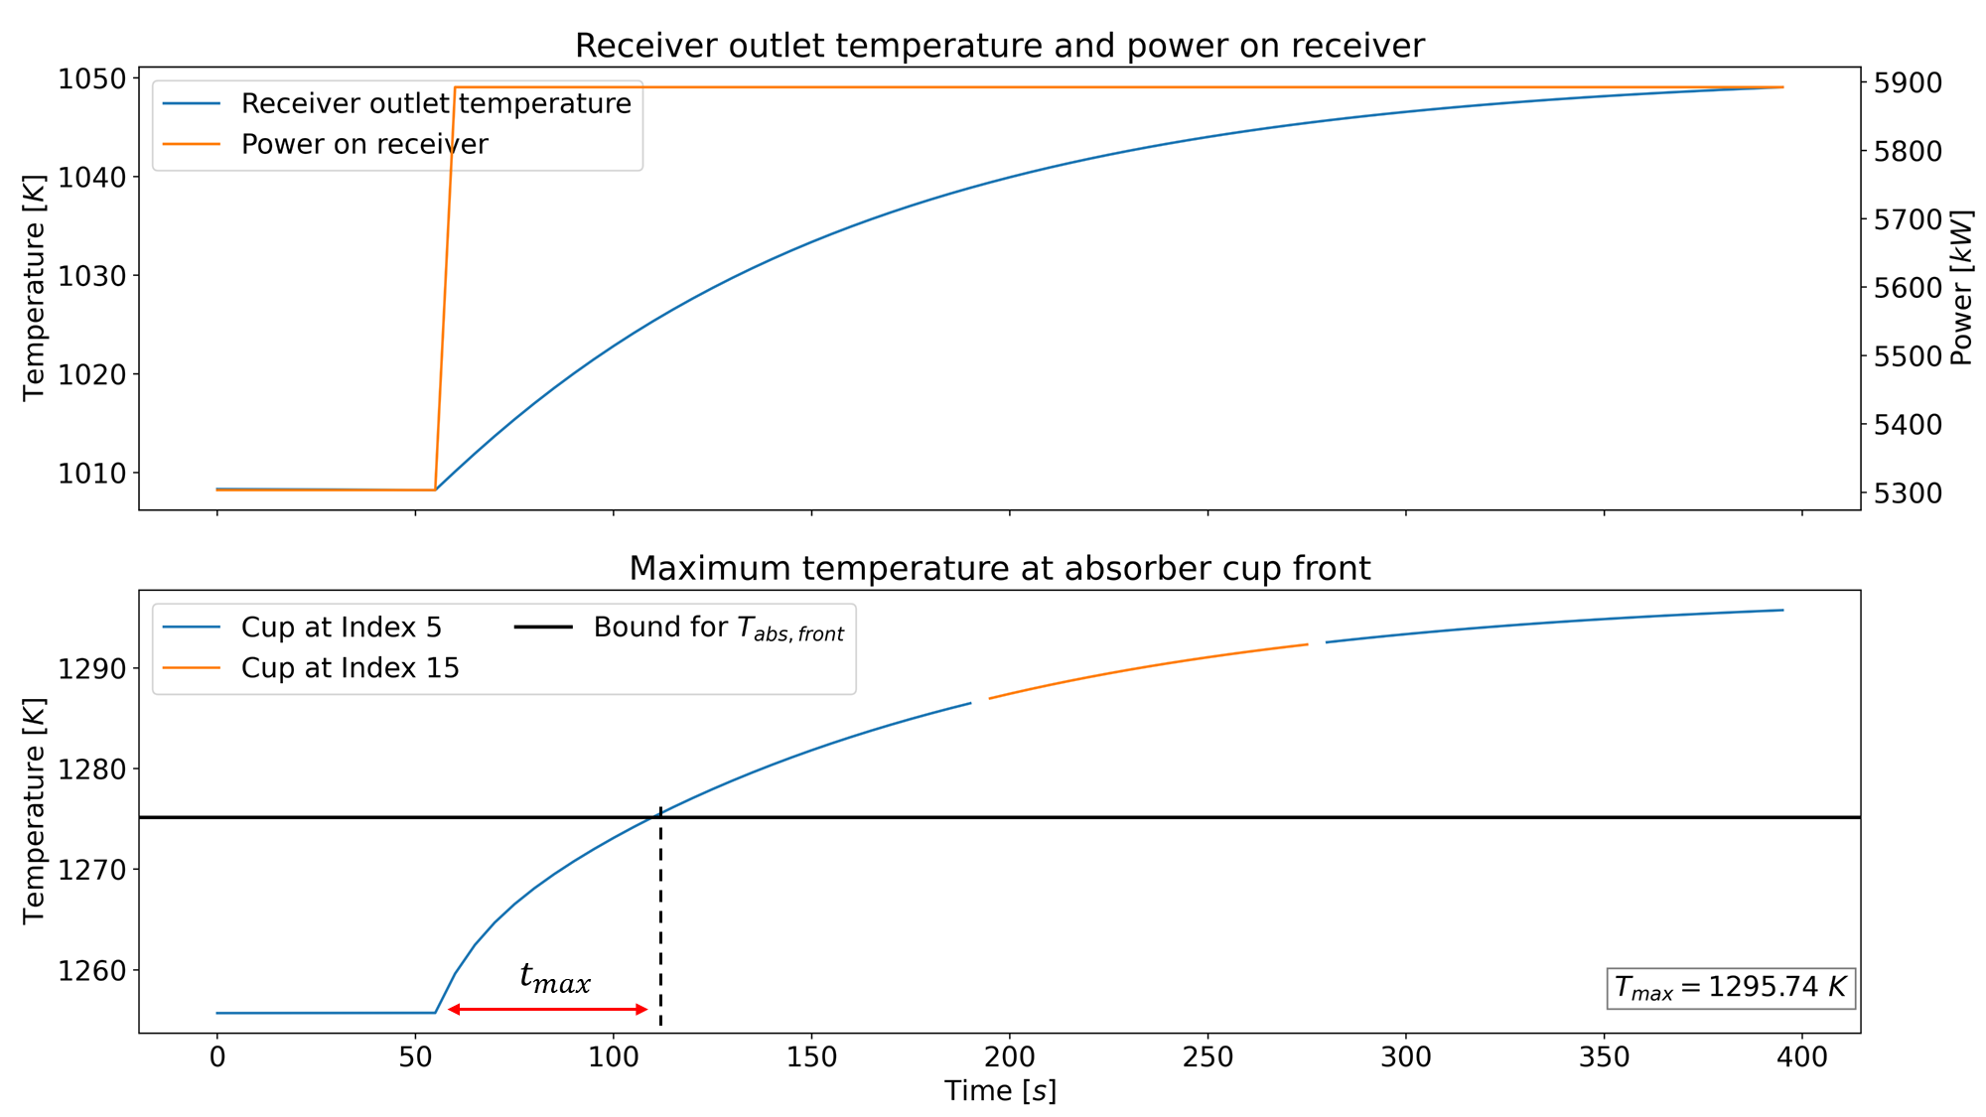
\includegraphics[width=0.99\textwidth]{C:/Users/gesc_ma/VSCode MPC Projekt/dynaovrcontroller/dynaovrcontroller/aimpoint_control_scenarios/plots/07_system_analysis/10prc_overflux_Temperatures_only_labeld.png}}
    \caption[Simulative Bestimmung der kritischen Zeit $t_{\mathrm{max}}$ bis zur Erhöhung der Receiver-Fronttemperatur um $\SI{10}{\kelvin}$]{Simulative Bestimmung der kritischen Zeit $t_{\mathrm{max}}$ bis zur Erhöhung der Receiver-Fronttemperatur um $\SI{20}{\kelvin}$}
    \label{fig_SampleTimebestimmen}
\end{figure}

Nach empirischer Analyse von Simulationen mit unterschiedlichen Abtastzeiten wird eine Abtastzeit von $T_s=\SI{10}{\second}$ gewählt.
Dies stellt einen akzeptablen Kompromiss zwischen einem zu hohen Berechnungsaufwand aufgrund kleiner Abtastzeiten und langsamer Reaktion des Reglers aufgrund zu großer Abtastzeiten dar.


\subsubsection*{Prädiktions- und Regelungshorizont} \label{subsubsec_horizonte}
Für die Dauer des Prädiktionshorizontes ist nach \cite{Bemporad} in erster Iteration die Ausregelzeit zu betrachten.
Auf diese Weise steht dem Regler zur Optimierung die gesamte Systemdynamik von der Anregung bis zum folgenden Gleichgewichtszustand zur Verfügung.
Daran angepasst kann der Kontrollhorizont bestimmt werden.
Dieser sollte $\SIrange{10}{20}{\percent}$ des Prädiktionshorizontes abdecken.

Gemäß Kapitel \ref{subsec_Systemdynamik} wird der Prädiktionshorizont zunächst mit der Ausregelzeit $T_{\mathrm{settling}} = N_{2,\mathrm{initial}} = \SI{450}{\second}$ angenommen.
Auf dieser Basis ergibt sich der obere Kontrollhorizont zu $N_u = 0.15\cdot N_{2,\mathrm{initial}} = \SI{60}{\second}$.
Der untere Kontrollhorizont $N_1$ wird gleich $0$ gesetzt, sodass der Regler in jeder Iteration die Stellgrößen verändern und schnell auf äußere Änderungen reagieren kann.
Da das Ziel der Arbeit die effektive Regelung bei kurzfristiger Änderung der solaren Einstrahlung darstellt, ist die Berechnung der Prädiktionen über einen Horizont von $\SI{7.5}{\minute}$ allerdings sehr hoch.
Um den Berechnungsaufwand zu verringern wird der Prädiktionshorizont dem Regelungshorizont angeglichen.
Daher gilt $N_2 = N_u = \SI{60}{\second}$.

\subsubsection*{Constraints} \label{subsubsec_constraints}
Gemäß dem Betriebshandbuch des Solarturmherstellers ist das Kraftwerk mit einem Luftmassenstrom im Bereich von $\SIrange{2.93}{11.7}{\kilo\gram\per\second}$ zu betreiben \cite[S.28]{HandbuchJülich}.
Der zulässige Bereich des Gebläse-Einstellwertes als Stellgröße des Reglers ist dementsprechend zu wählen (vgl. Kapitel \ref{subsec_BeschreibungLüftungsDyn}).
Durch die Diskretisierung des Systems auf 30 repräsentative Absorbercups nach Abschnitt \ref{sec_KopplungModelle} ergibt sich in der Simulation ein zulässiger Massenstrom von $\SIrange{80.82}{322.74}{\gram\per\second}$.
Dies entspricht einem Einstellwert von $\SI{227.5}{\metre\cubed\per\hour} \leq u_{\mathrm{setpoint}} \leq \SI{908.3}{\metre\cubed\per\hour}$.

Wie in Kapitel \ref{subsubsec_Gruppenverhalten} dargestellt, gilt für kleine Streuungsfaktoren eine Ausrichtung der Zielpunkte auf die Receivermitte.
Für größere Werte werden die Heliostaten defokussiert und die vom Receiver absorbierte Leistung sinkt.
Ein sinnvoller Rahmen der Defokussierung ergibt sich empirisch im Kontext des Modells zu $0 \leq \kappa \leq 50$.

Die vier Stellgrößen der Regelung werden gemäß Kapitel \ref{subsec_Constraints} als harte Limitierungen gewählt.
Im Rahmen der Optimierung können diese Variablen nur Werte innerhalb der jeweiligen Beschränkungen annehmen.
Dies ist notwendig, um die Betriebssicherheit des Kraftwerkes und die Sinnhaftigkeit der Lösungen der Optimierung zu gewährleisten.

Weiterhin ist bezüglich der Betriebssicherheit des Solarturmkraftwerkes zu sicherzustellen, dass die thermische Spannung in den Absorbercups den zulässigen Grenzwert nicht überschreitet.
Dazu darf die Fronttemperatur des Receivers $\TAbsorberFront~\SI{1002}{\celsius}$ nicht überschreiten \cite[S.29]{HandbuchJülich}.
Um die Lösbarkeit des Gleichungssystems der Regelung nicht zu gefährden (vgl. Kapitel \ref{subsec_Constraints}), wird zur Einhaltung dieser Temperatur eine weiche Limitierung bei $\SI{982}{\celsius}$ eingeführt.
Ein Überschreiten dieses Limits sorgt somit nicht automatisch für die Unlösbarkeit des Gleichungssystems.
Auch die Sicherheit des Absorbers ist bei Überschreitung dieses Wertes noch nicht gefährdet.

\subsubsection*{Kostenfunktion} \label{subsubsec_Kostenfunktion}
Die Kostenfunktion der Regelung ergibt sich nach dem in Gleichung \ref{eq_Optimierungsproblem} vorgestellten Muster.
Tabelle \ref{tab_Kostenfunktion} fasst alle Werte der verwendeten Größen zusammen:

\begingroup
\renewcommand{\arraystretch}{1.7}
\begin{table}[ht!]
    \caption[Übersicht über die Parameter zur Erstellung der Kostenfunktion]{Übersicht über die Parameter zur Erstellung der Kostenfunktion}
    \centering
    \begin{tabular}{>{\centering\arraybackslash}m{0.2\textwidth}>{\centering\arraybackslash}m{0.6\textwidth}}
        \rowcolor{white}
        \toprule
        Parameter der Kostenfunktion & Wert                                                                                                                                                                                \\
        \midrule
        $\boldsymbol{r}$             & $\SI{740}{\celsius}$                                                                                                                                                                \\
        $\boldsymbol{y}$             & $T_{\mathrm{out}}$                                                                                                                                                                  \\[-0.5cm]
        $\Delta \boldsymbol{u}$      & \vspace*{-0.5\baselineskip}\[\arraycolsep=0pt\def\arraystretch{1} \Delta \left(\begin{array}{c} \kappa_1 \\ \kappa_2 \\ \kappa_3 \\ u_{\mathrm{setpoint}} \end{array}\right) \] \\[-0.2cm]
        $\boldsymbol{\xi}$           & $
        \begin{cases}
                0                                    & \text{für } \TAbsorberFront \leq \SI{982}{\celsius} \\
                \TAbsorberFront - \SI{982}{\celsius} & \text{für } \TAbsorberFront > \SI{982}{\celsius}    \\
            \end{cases}$                                                                                                                         \\[0.4cm]
        $\boldsymbol{W_w}$           & $1$                                                                                                                                                                                 \\[-0.7cm]
        $\boldsymbol{W_u}$           & \[\arraycolsep=0pt\def\arraystretch{1.2} \left(\begin{array}{c} 10 \\ 10 \\ 10 \\ \SI{0.01}{} \end{array}\right) \]                                                                 \\[-0.5cm]
        $\boldsymbol{W_{\xi}}$       & $\SI{1e4}{}$                                                                                                                                                                        \\
        \toprule
    \end{tabular}
    \label{tab_Kostenfunktion}
\end{table}
\endgroup


Das stationäre Ziel der Regelung ist, die Temperatur des erwärmten Luftmassenstroms $T_{\mathrm{out}}$ als indirekte Modellausgangsgröße $\boldsymbol{y}$ der Referenz $\boldsymbol{r}$ von $\SI{740}{\celsius}$ anzupassen.
Dieser Referenzwert stellt die mittlere Luftaustrittstemperatur aus den Absorbermodulen im Nennlastpunkt dar \cite[\S.29]{HandbuchJülich}.
Während der Regelung wird zusätzlich die Änderung der Eingangsgrößen zwischen zwei Abtastzeitpunkten $\Delta \boldsymbol{u}$ betrachtet.
Die Slack Variable $\boldsymbol{\xi}$ kennzeichnet die Überschreitung der weichen Limitierungen.
Für den Fall, dass die Limitierung nicht überschritten wird, ergibt sich der Wert zu 0.
Die in der Kostenfunktion genutzten Gewichtungsmatrizen $\boldsymbol{W_w}$, $\boldsymbol{W_u}$ und $\boldsymbol{W_{\xi}}$ werden empirisch gewählt.


Das vollständige Optimierungsproblem der modellprädiktiven Regelung ergibt sich durch die Wahl der Diskretisierungsmethode gemäß Kapitel \ref{subsec_Diskretisierung}.
Demnach wird die orthogonale Kollokation mittels finiter Elemente angewandt.
Die Verteilung der Kollokationspunkte geschieht nach Legendre-Gauss-Radau (vgl. Abbildung \ref{fig_Kollokationspunkte}), die besonders bei sogenannten \gans{steifen} Systemen gute Ergebnisse erzielt \cite[S.178]{Diehl2}.
Gemäß \cite[S.171ff]{Diehl2} sind dies Systeme, bei denen verschiedene Systemdynamiken signifikante Unterscheide in ihren jeweiligen Zeitkonstanten aufweisen.

\section{Vorstellung der gesamten Regelung} \label{sec_VorstelungRegelung}
Eine Darstellung des vollständigen Regelkreises zeigt Abbildung \ref{fig_Regelkreisvollst}.
Die Rückführgrößen stellen die vier Systemzustände $\TAbsorberFront$, $\TAbsorberBack$, $\MDotReceiver$ und $\ddot{m}_{\mathrm{rec}}$ dar.
Es ist erkennbar, dass das Modell mit approximierten Flussdichtekarten der Optimierung dient, während das Modell mit den unveränderten Daten aus STRAL zur Simulation des Solarturms verwendet wird.
Weiterhin werden unterschiedliche Einstrahlungskarten des Nowcastings für die Optimierung und die Simulation verwendet.
Dies ist erforderlich, da sich Einstrahlungsprädiktionen in realer Anwendung von der tatsächlichen Einstrahlung unterscheiden.

\begin{figure}[h!]
   \centering
   \setlength{\fboxsep}{1pt}
   \setlength{\fboxrule}{1pt}
   \fbox{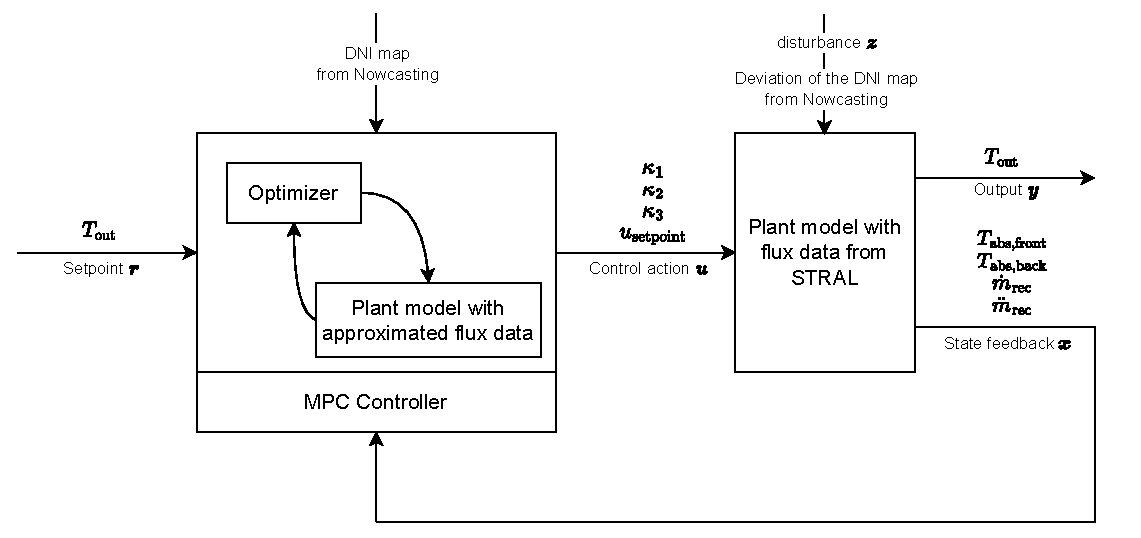
\includegraphics[width=0.99\textwidth]{fig/regelkreis_konkretessystem.pdf}}
   \caption[Vollständiger Regelkreis des Gesamtmodells inklusive aller Ein- und Ausgangsgrößen]{Vollständiger Regelkreis des Gesamtmodells inklusive aller Ein- und Ausgangsgrößen}
   \label{fig_Regelkreisvollst}
\end{figure}


\section{Übertragbarkeit auf das Realsystem} \label{sec_RealsystemRegelung}
In \cite[S.1]{Skogestad} wird im Rahmen der Systemanalyse auch die Betrachtung von Sensorik und Aktorik sowie erforderlichen Messgrößen vorgeschlagen.
Im Rahmen dieser Arbeit ist dies nicht erforderlich, da ein rein simulatives Modell betrachtet wird.
Für eine potenzielle Übertragung der Regelung auf den Solarturm ist diese Betrachtung jedoch essenziell und wird nachfolgend eingeführt.

Die Rückführgrößen der vorgestellten Regelung sind die Systemzustände, deren Messung am Solarturm in Jülich jedoch nicht vorgesehen ist.
Messbare Größen sind unter anderem die Flussdichteverteilung $F$ auf dem Receiver, die Fronttemperatur der Absorbercups $\TAbsorberFront$, die Austrittstemperatur des aufgeheizten Luftstroms an der Receiverinnenseite $T_{\mathrm{out}}$ und der Luftmassenstrom $\MDotReceiver$.
Zur Ermittlung der beiden fehlenden Zustände $\TAbsorberBack$ und $\ddot{m}_{\mathrm{rec}}$ wird daher ein Zustandsbeobachter benötigt.

Eine weitere Messgröße stellt, wie in Kapitel \ref{subsubsec_EnergiebilanzTransportzone} erwähnt, die Temperatur der Rückführluft $\TReturn{3}$ dar.
Simulativ wird diese als konstant angenommen, ist jedoch in der Realität von der Nutzung der erhitzten Luft abhängig.

Auch die Betrachtung expliziter Aktoren und Stellglieder sowie deren Eigenschaften entfällt simulativ.
Bei Regelung des Realsystems erweitert sich der Regelkreis jedoch um die Motoren der Heliostaten und der Pumpe.
